% --------------------------------------------------------------
% This is all preamble stuff that you don't have to worry about.
% Head down to where it says "Start here"
% --------------------------------------------------------------
 
\documentclass[12pt]{article}
 
\usepackage[margin=1in]{geometry}
\usepackage{amsmath,amsthm,amssymb}
\usepackage{hyperref}
\usepackage{graphicx}
\graphicspath{ {./images/} }
\usepackage{placeins}
\usepackage[export]{adjustbox}
 
\newcommand{\N}{\mathbb{N}}
\newcommand{\Z}{\mathbb{Z}}
 
\newenvironment{theorem}[2][Theorem]{\begin{trivlist}
\item[\hskip \labelsep {\bfseries #1}\hskip \labelsep {\bfseries #2.}]}{\end{trivlist}}
\newenvironment{lemma}[2][Lemma]{\begin{trivlist}
\item[\hskip \labelsep {\bfseries #1}\hskip \labelsep {\bfseries #2.}]}{\end{trivlist}}
\newenvironment{exercise}[2][Exercise]{\begin{trivlist}
\item[\hskip \labelsep {\bfseries #1}\hskip \labelsep {\bfseries #2.}]}{\end{trivlist}}
\newenvironment{problem}[2][Problem]{\begin{trivlist}
\item[\hskip \labelsep {\bfseries #1}\hskip \labelsep {\bfseries #2.}]}{\end{trivlist}}
\newenvironment{question}[2][Question]{\begin{trivlist}
\item[\hskip \labelsep {\bfseries #1}\hskip \labelsep {\bfseries #2.}]}{\end{trivlist}}
\newenvironment{corollary}[2][Corollary]{\begin{trivlist}
\item[\hskip \labelsep {\bfseries #1}\hskip \labelsep {\bfseries #2.}]}{\end{trivlist}}

 
\begin{document}
 
% --------------------------------------------------------------
%                         Start here
% --------------------------------------------------------------
 
\title{TMA4101 Matematikk 1 - Øvingsinnlevering}%overskrift
\author{Hanna Uche Arukwe & Tora Berntsen\\ %replace with your name
} %if necessary, replace with your course title
 
\maketitle\textbf{Newtons avkjørlingslov på en bakt potet}

\section{Ingress}
Poteten, den elskede...grønnsaken? Poteten kan brukes til så mangt og varmer hjertene til mennesker i alle aldre\footnote{\href{https://www.youtube.com/watch?v=r-L71ZNHRps} {Historien om den fantastiske poteten}}. Selv et barnehagebarn vet dette. Men hvor godt poteten greier å holde på varmen, var det ingen som lurte på, men vi testa det nå likevel. I tillegg til å sammenligne Newtons avkjølingslov med avkjøling av en potet i praksis, hadde vi også som mål å kose oss og  gripe muligheten til å lage tidenes bakt potet. 

\section{Metode}
Poteten ble varmet opp i stekeovn på 210$^{\circ}$ C i omtrent 90 minutter.  Deretter ble poteten "stabba" med et termometer og lagt i et rom med romtemperatur på omtrent 22$^{\circ}$ C. Potetens indre temperatur ble målt hvert 4. minutt.  Termometeret vi brukte viste kun temperaturen fra 95-55 grader, så vi fikk kun gjort målinger innenfor dette intervallet. . 
 
\section{Resultater}
Ved å bruke Newtons avkjølingslov bruker vi differansen mellom romtemperaturen, 22$^{\circ}$ C, og potetens indre temperatur  ved tidspunktet t, til å estimere hvordan potetens temperatur vil endre seg over tid. Vi brukte initialebetingelsene T(0) = 92$^{\circ}$ C og T(20) = 70$^{\circ}$ C, og kom med det fram til at proporsjonalitetskontantsen, \(\alpha\), er 
\(\frac{ln(48/70)}{20}\).

 \begin{figure} 
     \centering
     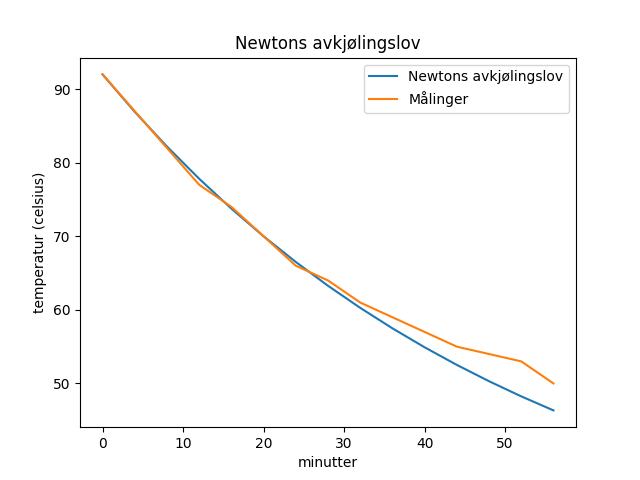
\includegraphics[width=0.75\linewidth]{tma4101 oblig kurver.png}
     \caption{Plot av teoretiske og målte verdier}
     \label{fig:enter-label}
 \end{figure}

\FloatBarrier
 
\section{Siste ord}
Som man kan se i plottet er Newtons avkjølingslov en god tilnærming til målingene til å begynne med, men vi får  større avvik etter ca. 30 minutter. Det hadde vært interessant å se hvordan målingene utviklet seg når temperaturen sank videre, men på grunn av vårt mangelfulle termometer fikk vi dessverre ikke gjort dette. Avvikene kan vi anta skyldes blant annet variasjon i romtemperaturen og andre faktorer Newtons avkjølingslov ikke tar hensyn til.  



\begin{figure}
    \centering
    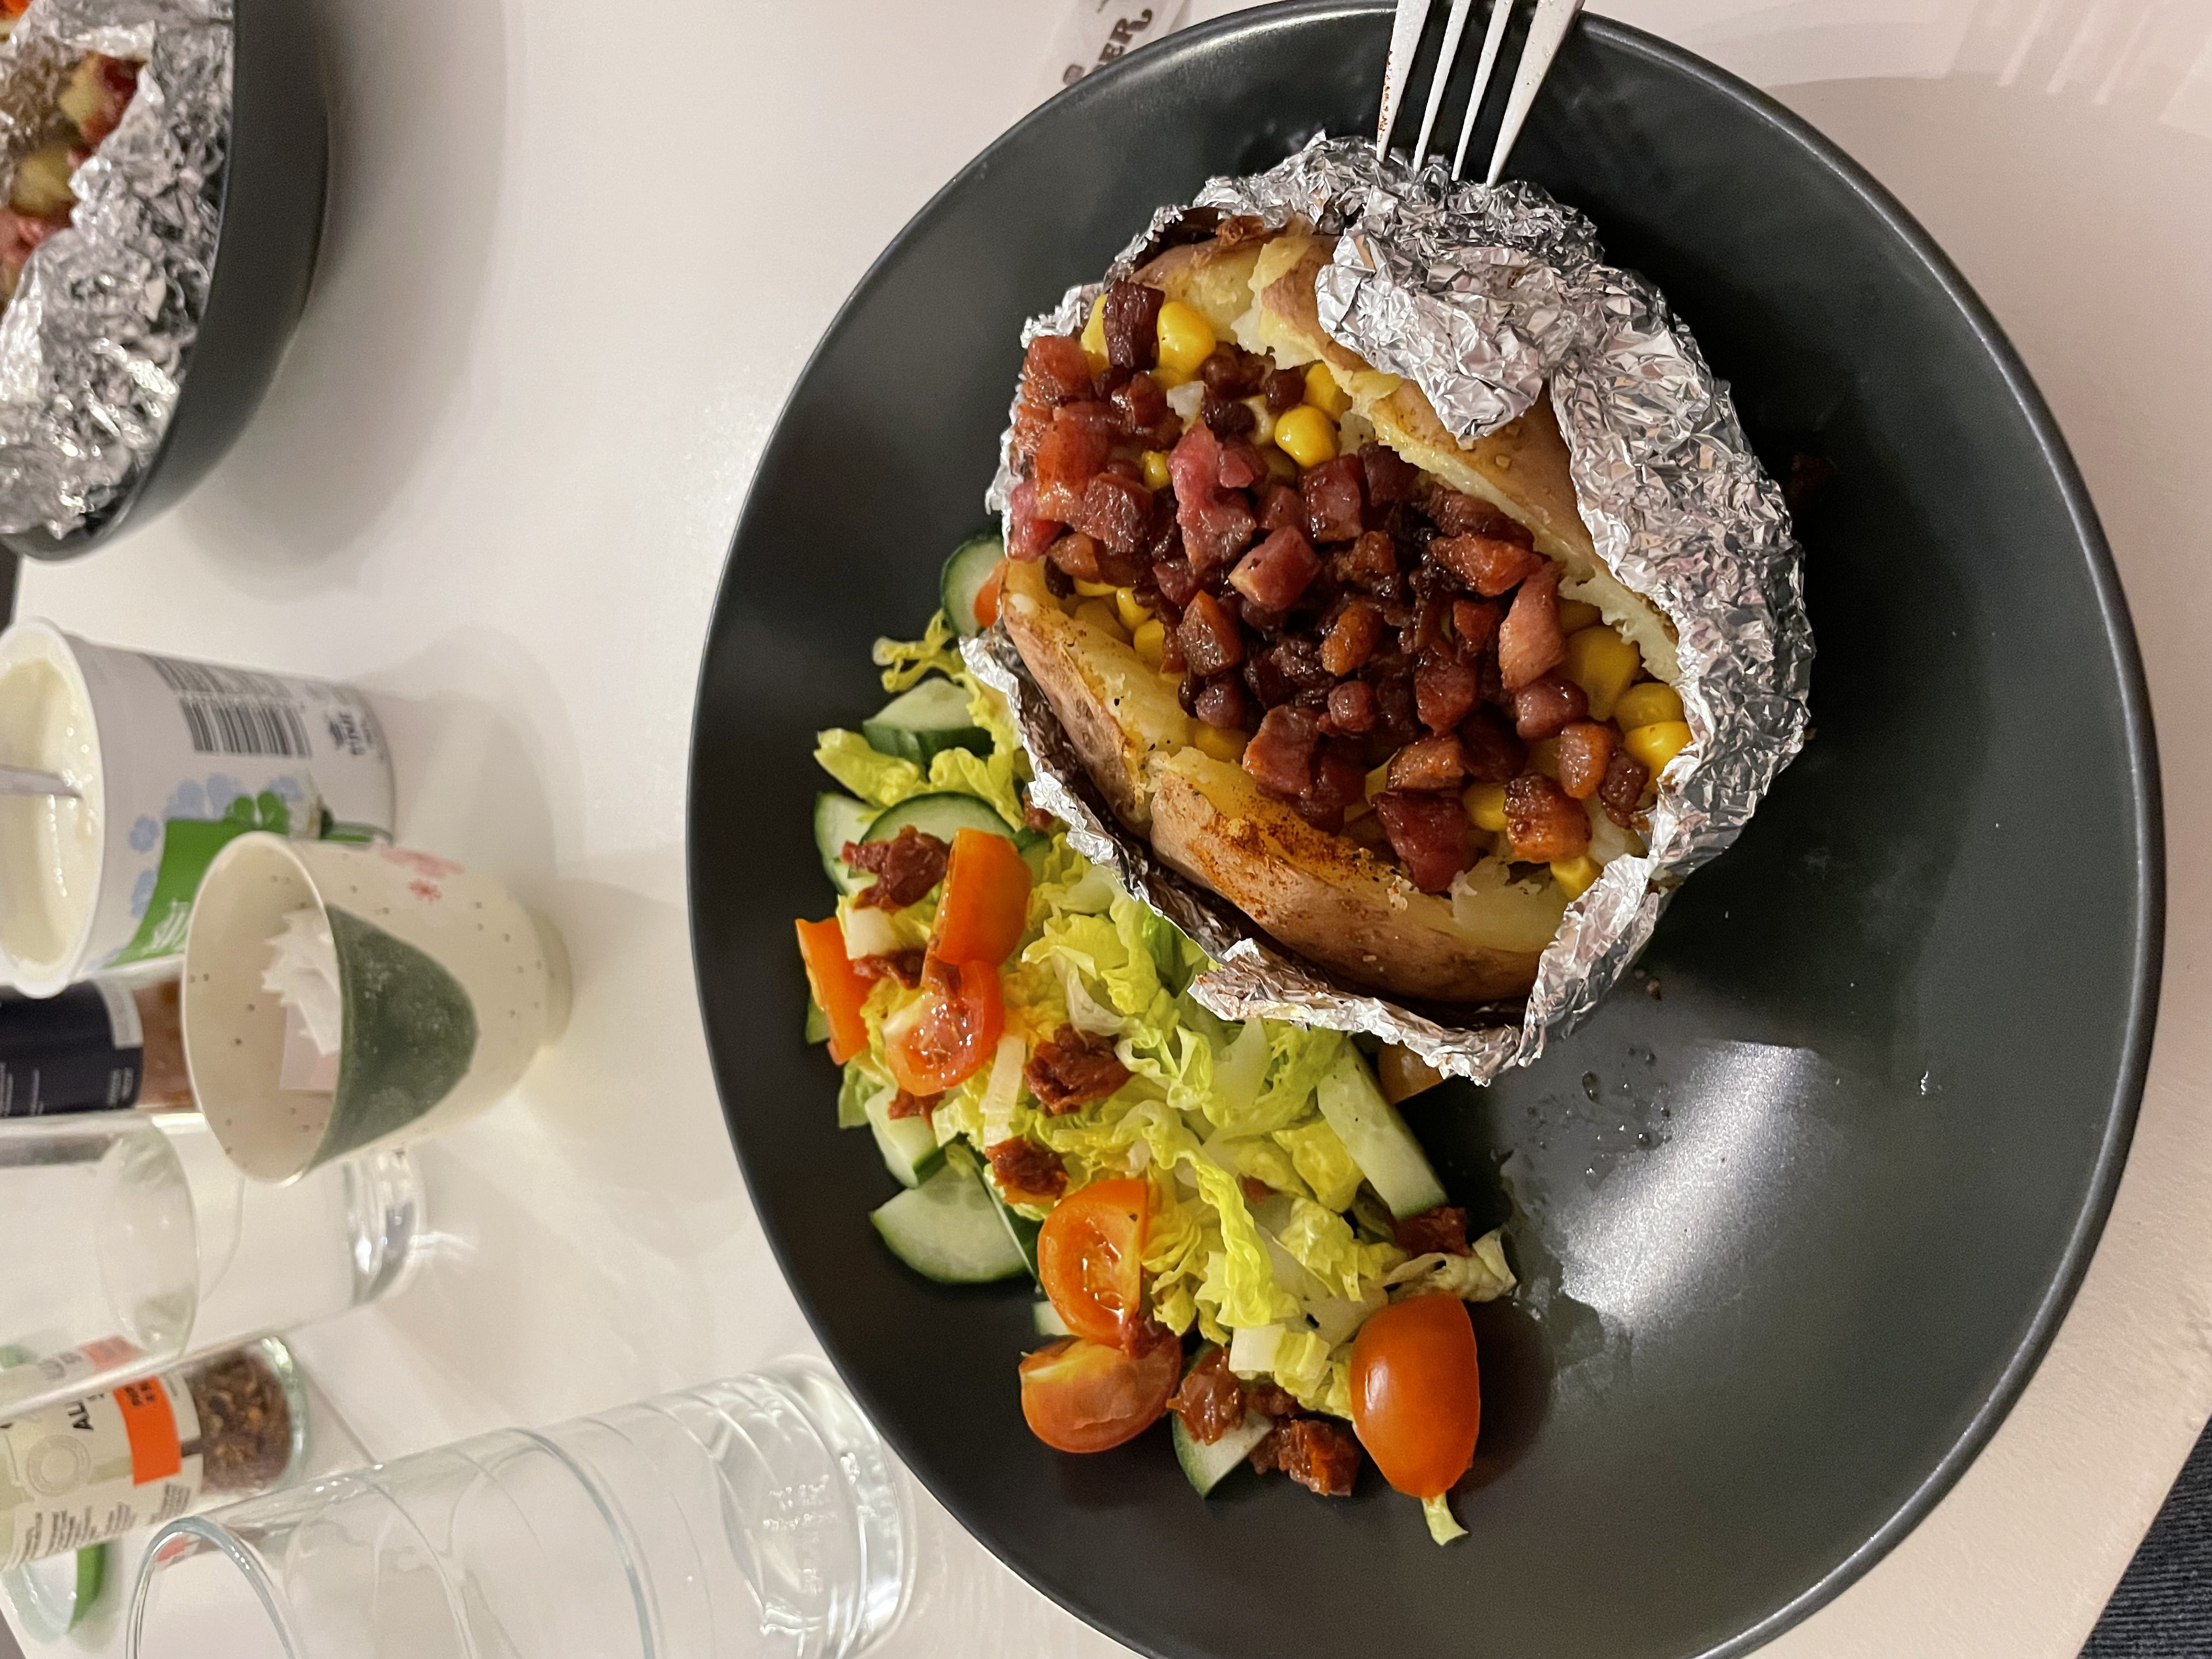
\includegraphics[width=0.50\linewidth, angle=-90]{image_67195393.JPG}
    \caption{What to not love her altså}
    \label{fig:enter-label}
\end{figure}

\FloatBarrier

Sivilingeniører er som poteten, tilpassningsdyktig og kan brukes til alt. Vi rate-er denne øvingsoppgaven 11/10 og den himmelske bakte poteten 100/10. Selv om mye tid gikk til å vente på at poteten ble varm, er vi begge enige om at det var verdt det. \textit{"De som venter på noe godt, venter ikke forgjeves}". 


 \begin{figure}[h]
     \centering
     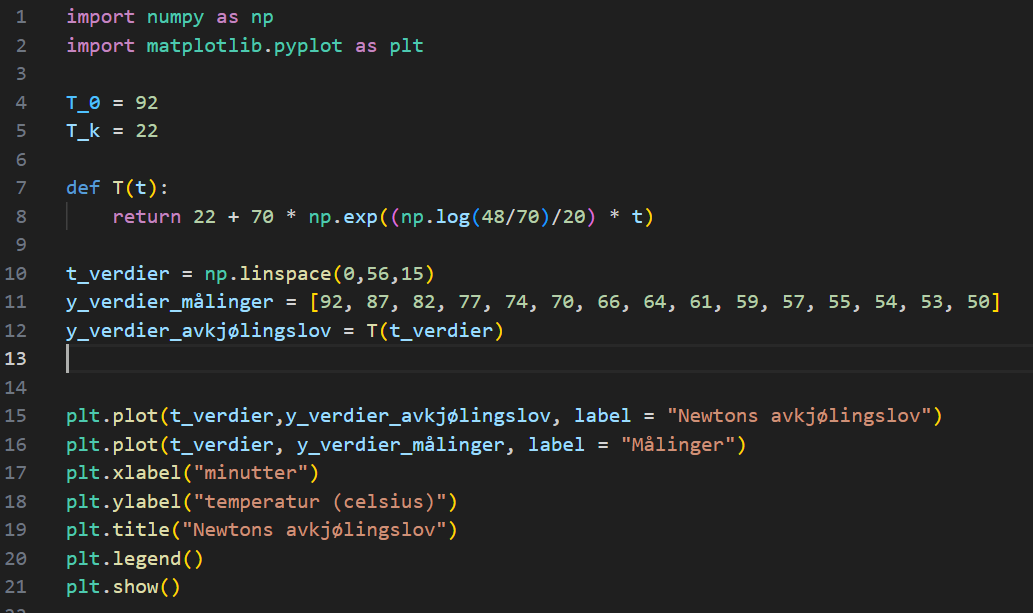
\includegraphics[width=0.5\linewidth ]{oblig kode.PNG}
     \caption{Kode for plotting}
     \label{fig:enter-label}
 \end{figure}
% --------------------------------------------------------------
%     You don't have to mess with anything below this line.
% --------------------------------------------------------------
 
\end{document}
